\chapter{知识表示方法}

\begin{question}
状态空间法、问题归约法、谓词逻辑法和语义网络法的要点是什么?它们有何本质上的联系及异同点?
\end{question}	
\begin{solution}
状态空间法:基于解答空间的问题表示和求解方法,它是以状态和算符为基础来表示和求解问题的。一般用状态空间法来表示下述方法:从某个初始状态开始,每次加一个操作符,递增的建立起操作符的试验序列,直到达到目标状态为止。 \par
问题规约法:已知问题的描述,通过一系列变换把此问题最终变成一个子问题集合:这些子问题的解可以直接得到,从而解决了初始问题。问题规约的实质:从目标(要解决的问题)出发逆向推理,建立子问题以及子问题的子问题,直至最后把出示问题规约为一个平凡的本原问题集合。 \par
谓词逻辑法:采用谓词合式公式和一阶谓词算法。要解决的问题变为一个有待证明的问题,然后采用消解定理和消解反演莱证明一个新语句是从已知的正确语句导出的,从而证明这个新语句也是正确的。\par
语义网络法:是一种结构化表示方法,它由节点和弧线或链组成。节点用于表示物体、概念和状态,弧线用于表示节点间的关系。语义网络的解答是一个经过推理和匹配而得到的具有明确结果的新的语义网络。语义网络可用于表示多元关系,扩展后可以表示更复杂的问题。
\end{solution}

\begin{question}
设有3个传教士和3个野人来到河边,打算成一条船从右岸渡到左岸去。该船的负载能力为两人。在任何时候,如果野人人数超过传教士人数,那么野人就会把传教士吃掉。怎样才能用这条船安全地把所有人都渡过河去?
\end{question}
\begin{solution}
\end{solution}

\begin{question}
利用××,用状态空间法规划一个最短的旅行路程:此旅程从城市A开始,访问其他城市不多于一次,并返回A。选择一个状态表示,表示出所求得的状态空间的节点及弧线,标出适当的代价,并指明图中从起始节点到目标节点的最佳路径。
\end{question}
\begin{solution}
\end{solution}

\begin{question}
试说明怎样把一棵与或解树用来表达图\ref{Fig:elec}所示的电网络阻抗的计算。单独的$R$、$L$或$C$可分别用$R$、$j\omega L$或$1/j\omega C$来计算,这个事实用作本原问题。后继算符应以复合并联和串联阻抗的规则为基础。
	\begin{figure}[h]
		\centering
		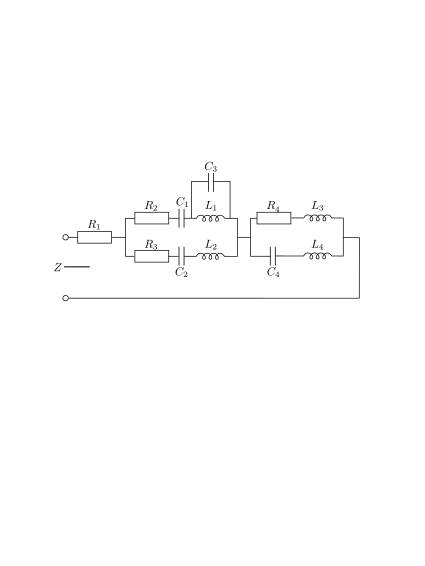
\includegraphics{ques-2.4.pdf}
		\caption{电网络阻抗计算} \label{Fig:elec}
	\end{figure}
\end{question}
\begin{solution}
\end{solution}

\begin{question}
试用四元数列结构表示四圆盘梵塔问题,并画出求解该问题的与或图。
\end{question}
\begin{solution}
\end{solution}

\begin{question}
把下列句子变换成子句形式:
	\begin{enumerate}
         \item $\left(\forall x\right) \left\{P\left(x\right) \to P\left(x\right)\right\}$
         \item $\forall x \forall y \left(\mathrm{On} \left(x,y\right) \to \mathrm{Above} \left(x,y\right) \right)$
         \item $\forall x \forall y \forall z \left(\mathrm{Above} \left(x,y\right) \wedge \mathrm{Above}\left(y,z\right) \to \mathrm{Above}\left(x,z\right) \right)$ 
         \item $\sim\left\{\left(\forall x\right)\left\{\left(\forall y)\left[p\left(y\right) \to p(f(x,y))\right] \wedge \left(\forall y \right) \left[Q(x,y) \to P(y) \right]\right\}\right\}\right\}$
	\end{enumerate}
\end{question}
\begin{solution}
\end{solution}

\begin{question}
用谓词演算公式表示下列英文句子(多用而不是省用不同谓词和项。例如不要用单一的谓词字母来表示每个句子)。
	\begin{quote}
		A computer system is intelligent if it can perform a task which, if performed by a human, requires intelligence. 
	\end{quote}
\end{question}
\begin{solution}
\end{solution}

\begin{question}
把下列语句表示称语义网络描述:
	\begin{enumerate}
		\item All men are moral.
		\item Every cloud has a silver lining.
		\item All branch manager of DEC participate in a profit-sharing plan. 
	\end{enumerate}
\end{question}
\begin{solution}
\end{solution}

\begin{question}
试构造一个描述你的寝室或办公室的框架系统。
\end{question}
\begin{solution}
\end{solution}

\begin{question}
框架和本体有何关系与区别?
\end{question}
\begin{solution}
\end{solution}